\documentclass{article}
\usepackage{graphicx} % Required for inserting images

\title{CONTROLOFALL}
\author{Someone Somewhere}
\date{April 20XX}

\begin{document}

\maketitle

\section{Abstract}

Mathematics is strange, a field simultaneously requiring only guarantees, yet at the same providing none.\\

Some mathematicians spend their whole lives working on a problem to fall just short of it. Some become known because of the problems they couldn't solve more than the ones that they could.\\

Mathematics is a love that wouldn't have worked out. Yet in my heart, remains that love. Perhaps it is that that I am still searching for.\\

Here is one last problem, the culmination of everything. The answers you seek lie in one number. But getting to it is not so simple. I have derived the path for you to walk, but I will not be the one to do so.\\

\section{A Path With No Guarantees}
\subsection{The beginning}
Let a circle $A$ exist of some radius $r$. Now let two circular arcs, members of some circles $B_1,B_2$ exist such that they lie tangent to $A$ on points $x=0$ and $y=r,-r$, and have radii of 8.\\

The points where $B_1$ and $B_2$ intersect are $(2\sqrt{7},0)$ and $(-2\sqrt{7},0)$ respectively.\\

The radius $r$ of $A$ is the number you need.\\
\begin{figure}
    \centering
    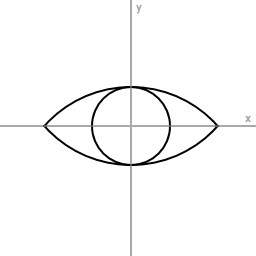
\includegraphics[width=0.5\linewidth]{CROSSOFTHEAXIS.png}
    \caption{CROSS OF THE AXIS}
    \label{fig:enter-label}
\end{figure}
\subsection{Recursion}
The fibonacci sequence is a set of numbers defined by the following rules:
\[F_0=0\]
\[F_1=1\]
\[F_n=F_{n-1} + F_{n-2}\]

There exists numbers $k$ such that that for all integers $z$, $F_{zk}$ is even. The smallest such number $k$ is your answer.\\

\subsection{A Hint From the Past}
The gamma function $\Gamma(x)$ is an extended definition of the factorial for all numbers except the negative integers. It is equivalent to $(x-1)!$ on positive integer inputs.\\

There is a single positive value of $x$ for which $\Gamma(x-1)=\Gamma(x+1)$. This value contains a square root, the answer to this puzzle is the integer under that square root.\\

\textit{Remark:} Important to note, whatever you do with these numbers, this one is twice as important.\\

\subsection{And around and around I go! :3}
What is the last digit of $3^{39916811}$?\\

\subsection{And yet I wont be found!}
What is the largest positive integer $k$ such that $k\neq20n+49m$ for any integers $n,m$?
%Compute the following:
%\[911^{39916801}\]
%Modulo 1000

\subsection{Big Things Await}
Let a lemniscate described by $r^2=1083\sin(2\theta)$ exist. How much area does it enclose?\\

Your answer here is found by $x^5 - 8,777,941,352$ where $x$ is the solution to the above problem\\

\section{Conclusion}
These numbers are the building blocks of mathematics - primes. With them you can construct all of the beauty this world has offered us.\\

You may think it is just a number, but if you get down to it, isn't everything in this world of wonderous technologies? Even the text on your screen.\\

Every day I wonder what could have been had I not done this path. What will things look like? There is a branch of math that deals with this stuff you know, Chaos Theory. The study of systems that significantly change under mildly small perturbations. Not knowing is perhaps part of the fun.\\

I'll be happy with who I am, and I'm sure I will be had I chose a different path instead.\\

\end{document}
